\subsection{Registries}

Having completed the work of generalizing access control and building access
control lists, we now introduce a simplified access control model for managing
voter registration during elections.

\begin{enumerate}
  \item \sol{interface Registry}, which defines the functions for registering
    voters for an election, and
  \item \sol{contract VoterRegistrationAuthority}, which implements and
    aggregates several \solt{interface}[s] and \solt{interface} implementations
    --- namely \sol{interface Registry}, \sol{interface Authority}, and
    \sol{contract ACLAuthority} --- to build a trusted source of registered
    voters.
\end{enumerate}

\begin{figure}[H]
  \centering
  \figurepdf[]{registry}
  \caption{Simplified election registry.}\label{fig:registry}
  % 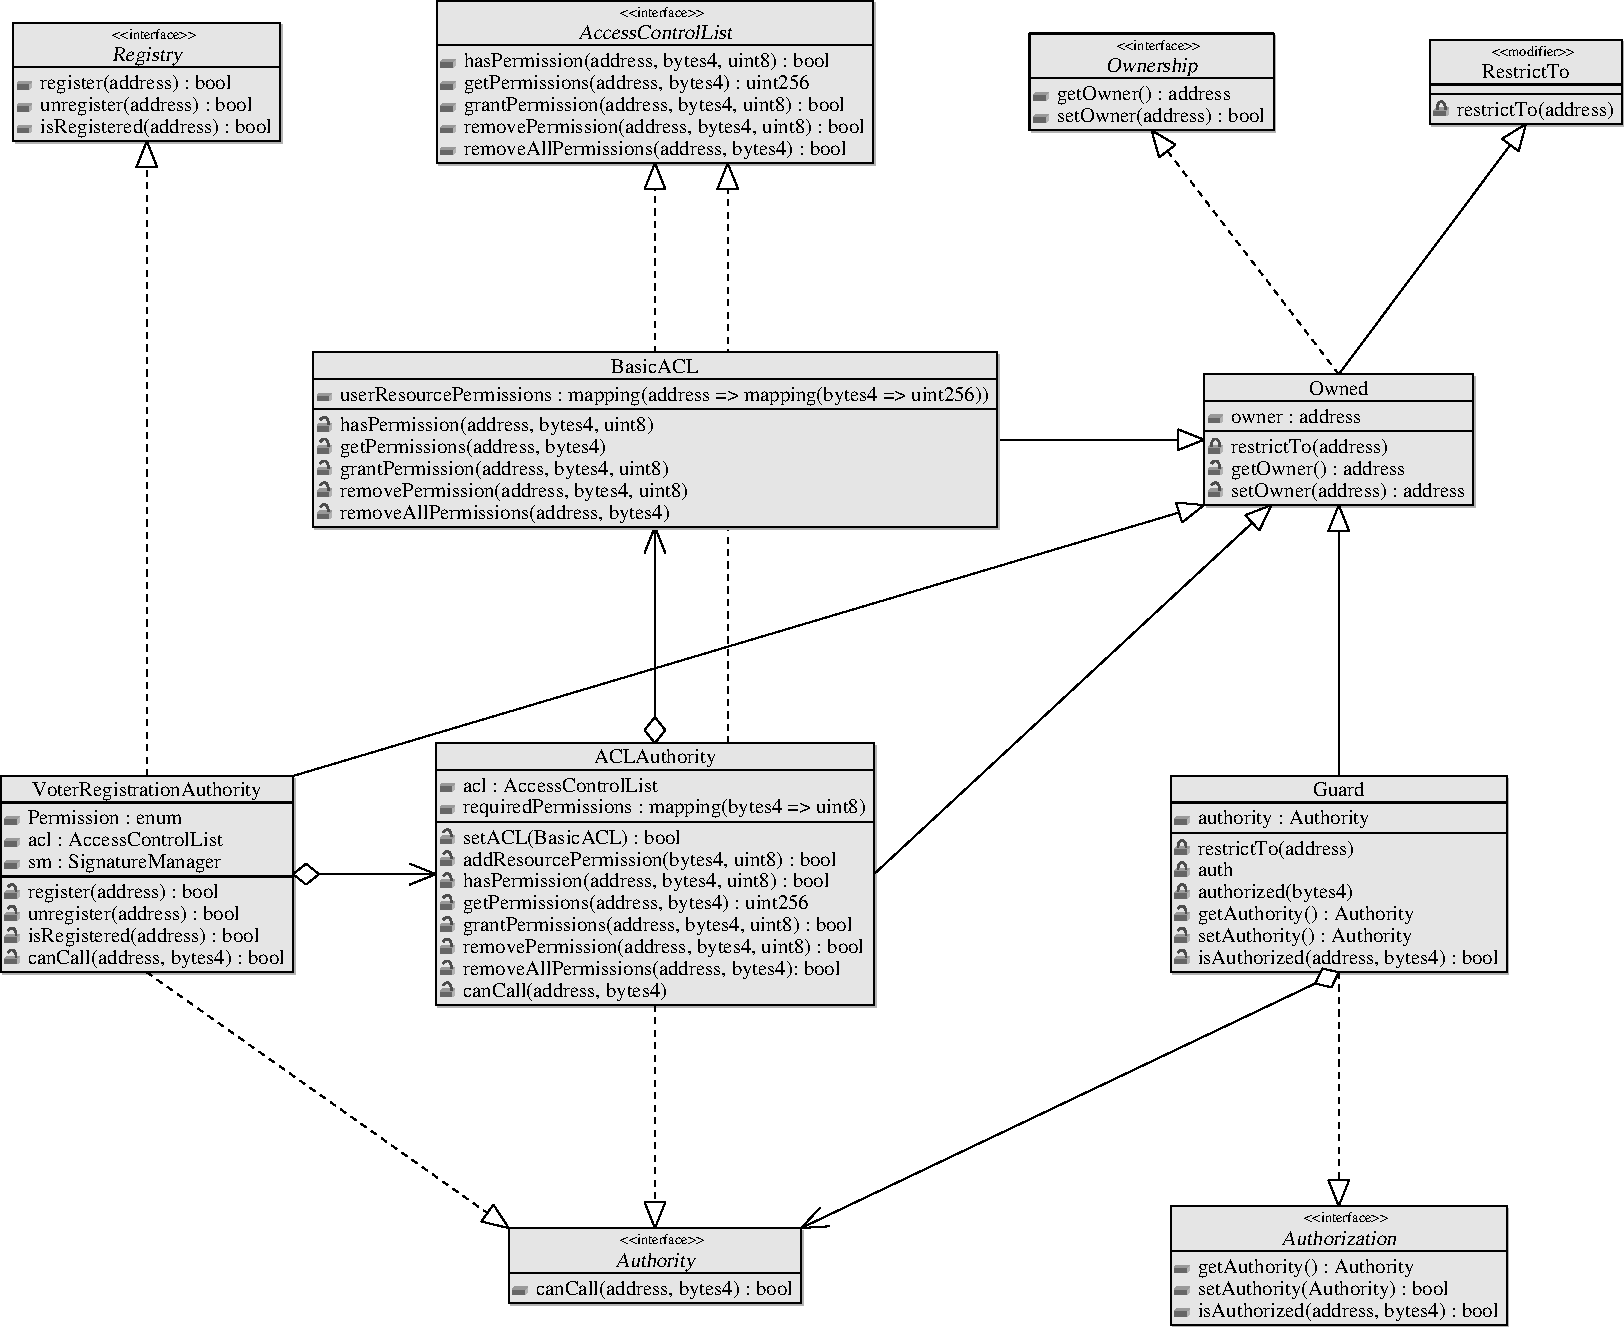
\includegraphics[width=\textwidth]{figures/authorization/figure}
  % \includestandalone[width=\textwidth]{\fig{authorization}}
\end{figure}

\subsubsection{Interface Registry}

The \solt{interface}, \sol{interface Registry}, introduces three \solt{function}
definitions required to achieve basic registry functionality:

\begin{enumerate}
  \item \sol{function register}, which \emph{registers} a \emph{subject}.

  \item \sol{function unregister}, which \emph{unregisters} a \emph{subject}.

  \item \sol{function isRegistered}, which evaluates whether a \emph{subject} is
    \emph{registered}.
\end{enumerate}

\begin{solidity}[interface Registry]
interface Registry {
  function register (address _subject) public returns (bool _success);
  function unregister (address _subject) public returns (bool _success);
  function isRegistered (address _subject) public constant returns (bool _isRegistered);
}
\end{solidity}

\begin{interface}
  \begin{functions}
    \item \sol{function isRegistered (address _subject)}, evaluates whether some
      \emph{subject} is \emph{registered}.

      \begin{parameters}
        \item \sol{address _subject}, the \solt{address} of an account
          representing the \emph{subject}, to evaluate the \emph{registration}
          of.
      \end{parameters}

      \begin{returns}
        \item \sol{bool _isRegistered}, returns the \solt{true} if the
          \emph{subject} is \emph{registered}, otherwise \solt{false}.
      \end{returns}

    \item \sol{function unregister (address _subject)}, \emph{unregisters} a
      \emph{subject}.

      \begin{parameters}
        \item \sol{address _subject}, the account \solt{address} of the
          \emph{subject} who is to be \emph{unregistered}.
      \end{parameters}

      \begin{returns}
        \item \sol{bool _success}, resolves to \solt{true} if the operation was
          successful, otherwise \solt{false}.
      \end{returns}

    \item \sol{function register (address _subject)}, \emph{registers} a
      \emph{subject}.

      \begin{parameters}
        \item \sol{address _subject}, the account \solt{address} of the
          \emph{subject} who is to be \emph{registered}.
      \end{parameters}

      \begin{returns}
        \item \sol{bool _success}, resolves to \solt{true} if the operation was
          successful, otherwise \solt{false}.
      \end{returns}
  \end{functions}
\end{interface}


\subsubsection{Contract VoterRegistrationAuthority}

The \solt{contract}, \sol{contract VoterRegistrationAuthority}, is the final
component of our authorization design and is required to construct a generalized
voter registration authority capable of managing registered voters and
conducting elections.

% signatureMap['vote'] = bytes4(sha3('vote(uint8[],uint8[])'));
\begin{solidity}[contract VoterRegistrationAuthority]
contract VoterRegistrationAuthority is Owned, Registry, Authority {
  enum Permissions {
    Vote
  }

  AccessControlList acl;
  mapping (bytes32 => bytes4) resourceSignatures;

  constructor () public {
    acl = new ACLAuthority(true);

    resourceSignatures['vote'] = bytes4(sha3('vote()'));

    acl.setRequiredResourcePermission(
      resourceSignature('vote'),
      uint8(Permissions.Vote)
    );
  }

  function register (address _voter) public restrictTo(owner) returns (bool _success) {
    return acl.grantPermission(_voter, resourceSignatures['vote'], uint8(Permissions.Vote));
  }

  function unregister (address _voter) public restrictTo(owner) returns (bool _success) {
    return acl.revokePermission(_voter, resourceSignatures['vote'], uint8(Permissions.Vote));
  }

  function isRegistered (address _voter) public constant returns (bool _isRegistered) {
    return acl.hasPermission(_voter, resourceSignatures['vote'], uint8(Permissions.Vote));
  }

  function canCall (address _subject, bytes4 _resource) public constant returns (bool _canCall) {
    return acl.canCall(_subject, _resource);
  }
}
\end{solidity}

\todo{Finish documenting the VoterRegistrationAuthority implementation.}

\begin{state}
  \begin{public}
    \item \sol{AccessControlList acl} maintains the \solt{address} of an ACL
      implementation, a \solt{contract} which implements \sol{interface
      AccessControlList}.

    \item \sol{mapping (bytes32 => bytes4) resourceSignatures} maintains a
      mapping of strings, \sol{bytes32}, to \solt{function} signature,
      \sol{bytes4}.
  \end{public}
\end{state}

\begin{code}
  \begin{constructor}
    \item \sol{constructor ()}, upon creation and initialization of this
      \solt{contract} the \solt{constructor} will deploy a \solt{contract},
      \sol{contract BasicACL}.
  \end{constructor}

  \begin{functions}
    \item \sol{function isRegistered (address _subject)}, evaluates whether some
      \emph{subject} is \emph{registered}.

      \begin{parameters}
        \item \sol{address _subject}, the \solt{address} of an account
          representing the \emph{subject}, to evaluate the \emph{registration}
          of.
      \end{parameters}

      \begin{returns}
        \item \sol{bool _isRegistered}, returns the \solt{true} if the
          \emph{subject} is \emph{registered}, otherwise \solt{false}.
      \end{returns}

    \item \sol{function unregister (address _subject)}, \emph{unregisters} a
      \emph{subject}.

      \begin{parameters}
        \item \sol{address _subject}, the account \solt{address} of the
          \emph{subject} who is to be \emph{unregistered}.
      \end{parameters}

      \begin{returns}
        \item \sol{bool _success}, resolves to \solt{true} if the operation was
          successful, otherwise \solt{false}.
      \end{returns}

    \item \sol{function register (address _subject)}, \emph{registers} a
      \emph{subject}.

      \begin{parameters}
        \item \sol{address _subject}, the account \solt{address} of the
          \emph{subject} who is to be \emph{registered}.
      \end{parameters}

      \begin{returns}
        \item \sol{bool _success}, resolves to \solt{true} if the operation was
          successful, otherwise \solt{false}.
      \end{returns}
  \end{functions}
\end{code}

